\documentclass{lecture}

\title{Neuro-symbolic integration}
\subtitle{Intro}
\author{Jedrzej Potoniec}

\graphicspath{{01_intro}}

\begin{document}

\frame{\titlepage}

\begin{frame}{Who am I?}
\begin{itemize}
\item an assistant professor in the Laboratory of Machine Learning;
\item interested in combining machine learning with complex data structures, in particular, neurosymbolic systems;
\item \url{www.cs.put.poznan.pl/jpotoniec}
\item \texttt{jedrzej.potoniec@cs.put.poznan.pl}
\item Office hours: see the address book (\url{https://informator.put.poznan.pl/})
\end{itemize}
\end{frame}

\begin{frame}{The goal of the course}
    \begin{itemize}
        \item to introduce you to an exciting, yet underdeveloped topic;
        \item to give you some breathing room to pursue something interesting, yet not necessarily immediately useful;
        \item to allow me to achieve better synergy between my research and teaching.
    \end{itemize}
\end{frame}

\begin{frame}{Schedule}
    \begin{enumerate}
        \item Intro to neuro-symbolic integration
        \item Reason-able embeddings
        \item Latplan        
        \item[4--7] Presentations of the recent advancements in the area
    \end{enumerate}
\end{frame}

\begin{frame}{Presentations}
    \begin{itemize}
        \item 20-minute talk about a paper published in the last two years (2022, 2023, 2024);
        \item containing neurosymbolic component
        \item you must get my approval for it \alert{before the talk}
        \item optionally: a team of $n\in\{1,2,3,4\}$ students presenting a single paper during a slot of $20n$ minutes        
    \end{itemize}
\end{frame}

\begin{frame}{Grading}
    \begin{itemize}
        \item A good talk fitting well into the slot will be granted the full mark. \item Talks too short, talks where the speaker doesn't know the topic well, etc. will be graded accordingly.
    \end{itemize}
\end{frame}

\begin{frame}{Project}
    You plan and execute a project where the core focus is on a neuro-symbolic component:
    \begin{itemize}
        \item A replication study. (the default)
        \item A part of your master's thesis.
        \item Your own idea.        
        \item My own idea (see the next lecture).
    \end{itemize}
\end{frame}

\begin{frame}{Workflow}
    \begin{enumerate}
        \item Discuss the scope with me during the project classes
        \item Submit a project proposal via eKursy, receive my approval
        \item Execute the project
        \item Submit a report (Monday before the defense)
        \item Defend the project
    \end{enumerate}
\end{frame}

\begin{frame}{Teams}
    \begin{itemize}
        \item default: 1 or 2 people per project
        \item more: convince me
    \end{itemize}
\end{frame}

\begin{frame}{Replication studies}
    If enough of you decide to make replication studies, we can compile your reports into a single paper and put it to arXiv.
\end{frame}

\begin{frame}{Timeline for the project}
    \begin{description}
        \item[28.02 -- 13.03] discussion phase;
        \item[13.03] project proposal submitted;
        \item[20.03 -- 10.04] first checkpoint;
        \item[17.04 -- 08.05] second checkpoint; 
        \item[15.05 -- 29.05] third checkpoint;
        \item[03.06/09.06] project report submitted;
        \item[05.06/12.06] project defense.
    \end{description}
\end{frame}

\begin{frame}{Project classes}
    \begin{itemize}
        \item three (or more) informal progress presentations
        \item public
        \item show progress; lack of it = lower grade                        
    \end{itemize}    
\end{frame}

\begin{frame}{Attendance}
    \begin{itemize}
        \item Mandatory to the extent given in the University's regulations.
        \item By itself doesn't influence your grades.
        \item Attend as little or as often as you like
    \end{itemize}
\end{frame}

\begin{frame}{On grading in general}
    This course is given 2 ECTS points. I am thus demanding little -- in principle, you give a short talk about a paper, play with whatever neurosymbolic thing you want, and summarize the results of that play.

    However, we are not playing the same game again where you pretend you didn't understand what \alert{beforehand} or \alert{my approval} means.
\end{frame}

\begin{frame}{Questions}
    \centering \Huge \alert{?}
\end{frame}

\begin{frame}{What is a neuro-symbolic system?}
    \begin{block}{Too narrow an answer}
        The combination of deep learning and symbolic reasoning
        \source{\url{https://arxiv.org/pdf/2012.05876.pdf}}
    \end{block}
    \pause
    \begin{block}{Perhaps too board an answer}
        Any system involving the manipulation of discrete (symbolic) and continuous (sub-symbolic) objects to achieve a shared goal
    \end{block}
    \pause
    \begin{block}{Not an answer}
        Not limited to knowledge graphs, logics, the Semantic Web, etc.
    \end{block}
\end{frame}

\begin{frame}{Why?}
    \begin{block}{Kahneman @ AAAI-20}
        (...) as far as I’m concerned, System 1 certainly knows the language (...)
System 2 does involve certain manipulation of symbols (...)
    \end{block}
    \source{\url{https://vimeo.com/390814190?ref=tw-share}}
\end{frame}

\begin{frame}{Strengths and weaknesses}
    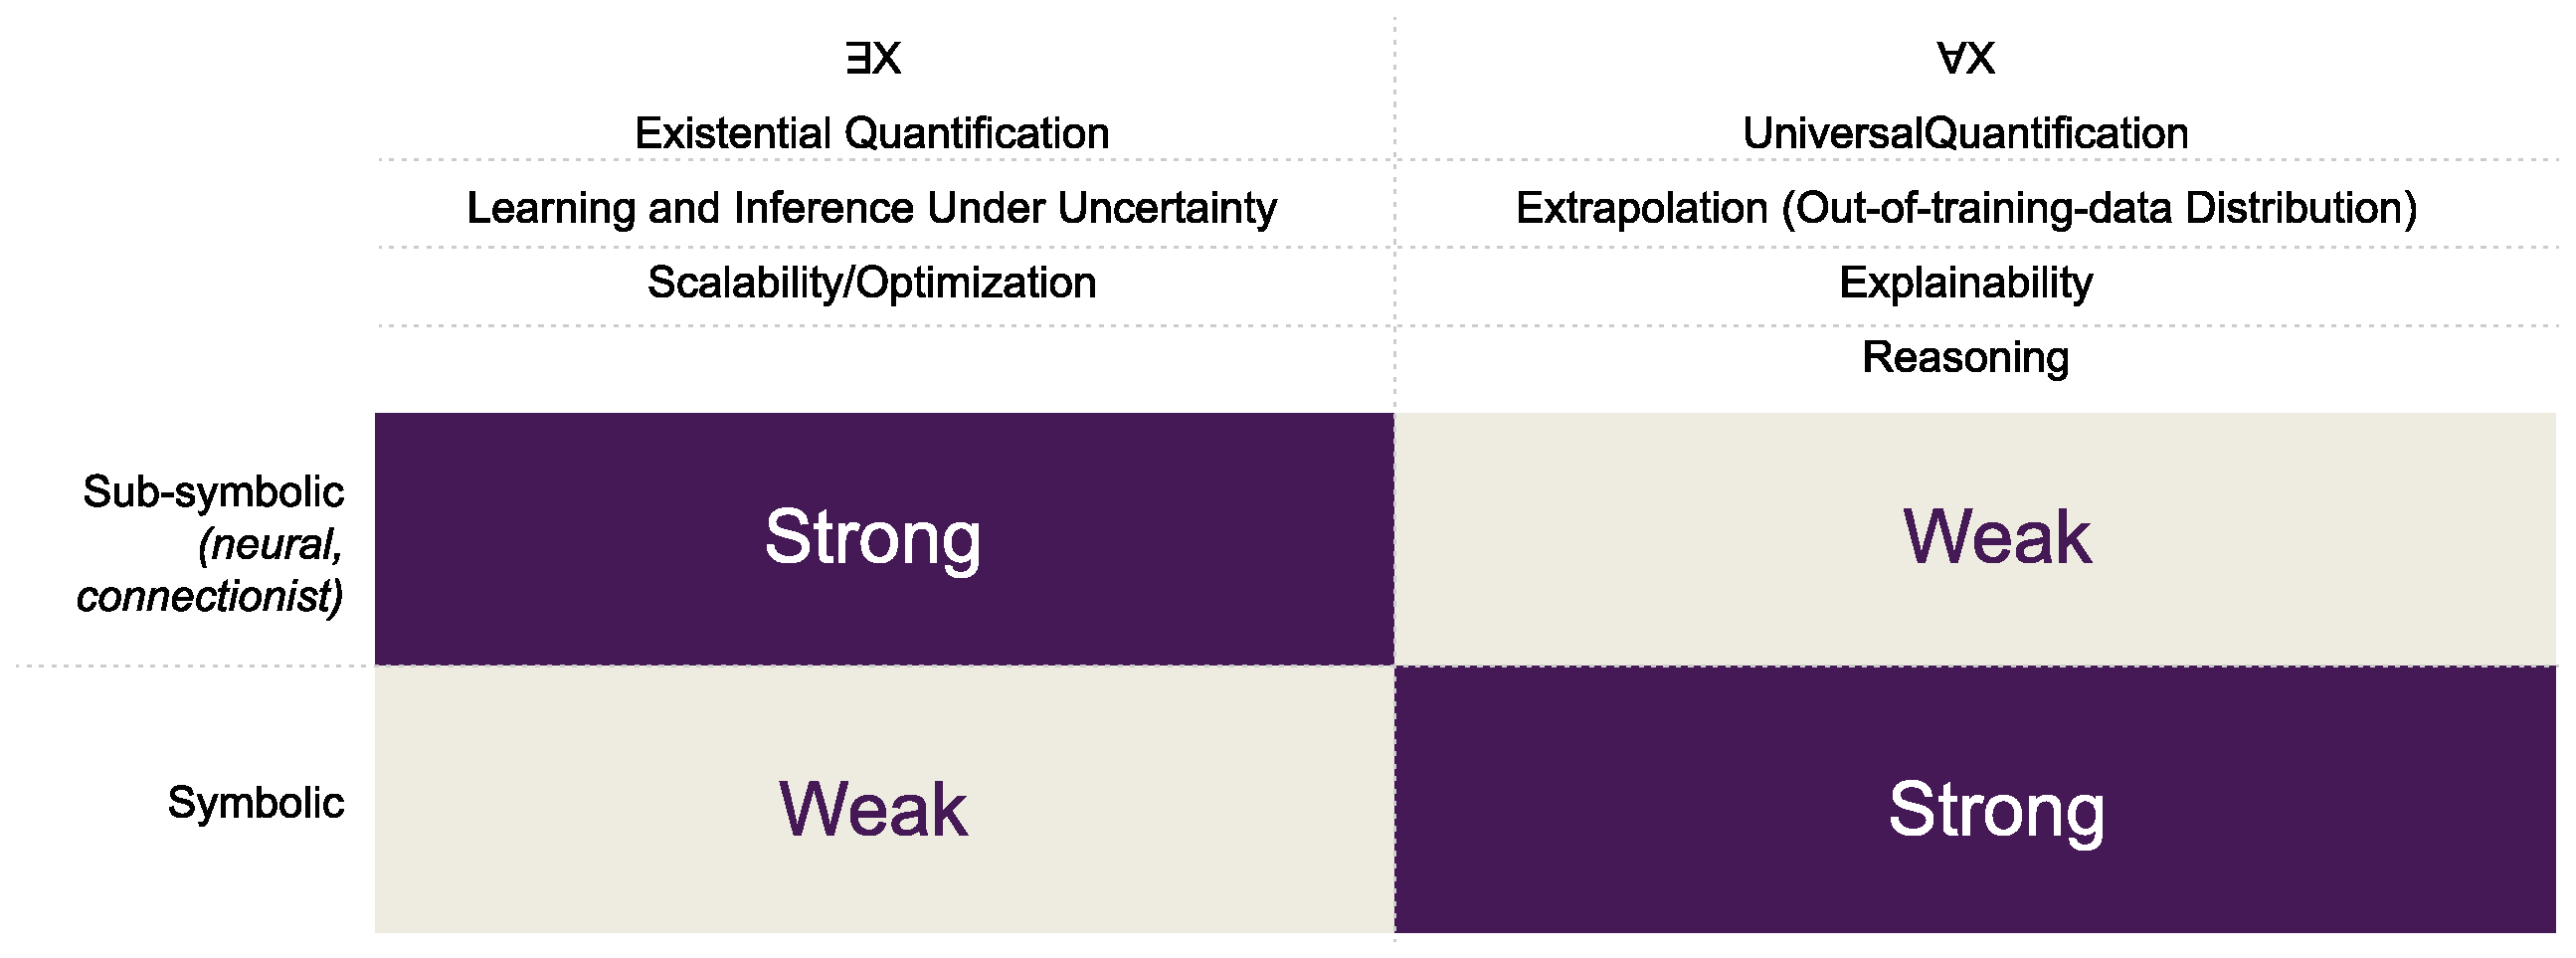
\includegraphics[width=\textwidth]{SW223228/nesy-table-diagram.eps}
    \source{\doi{10.3233/SW-223228}}
\end{frame}

\begin{frame}{Promises}
    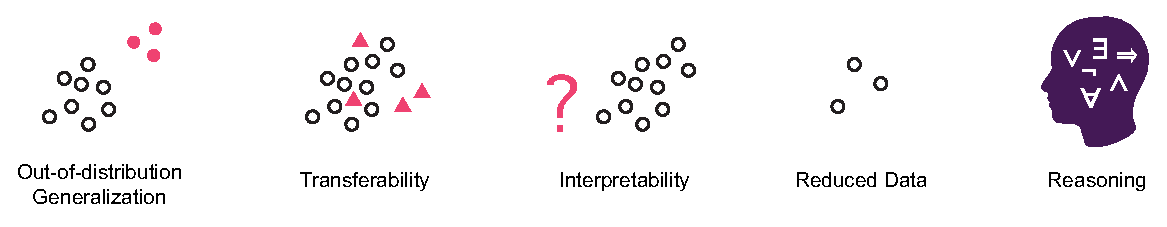
\includegraphics[width=\textwidth]{SW223228/promises.eps}
    \source{\doi{10.3233/SW-223228}}
\end{frame}


\begin{frame}{It is relevant for bussiness}
    ROAD-R contains 22 carefully selected, relatively long-duration (~8 minutes each) videos (\ldots) annotated with road events (\ldots). Road events are defined as a series of bounding boxes linked in time annotated with:

    \begin{itemize}
        \item the label associated to the agent (e.g., “Pedestrian”),
        \item the action(s) the agent is doing (e.g., “Pushing Object”, “Moving Away”), and
        \item the location(s) where the agent is placed (e.g., “Right Pavement”, “Bus Stop”).
    \end{itemize}
    (\ldots)

Furthermore, ROAD-R comes with \alert{243 logical requirements asserting which sets of labels can be associated with the bounding boxes}. The requirement "not MoveAway or not MoveForward", for example, expresses the fact that an agent cannot move away and towards the vehicle at the same time. 
    \source{\url{https://sites.google.com/view/road-r/home}}
\end{frame}

\begin{frame}{It is relevant for bussiness}
    We see Neuro-symbolic AI as a pathway to achieve artificial general intelligence. By augmenting and combining the strengths of statistical AI, like machine learning, with the capabilities of human-like symbolic knowledge and reasoning, we're aiming to create a revolution in AI, rather than an evolution.

\source{\url{https://research.ibm.com/topics/neuro-symbolic-ai}}
\end{frame}


\begin{frame}{It is gaining popularity}
    \centering
    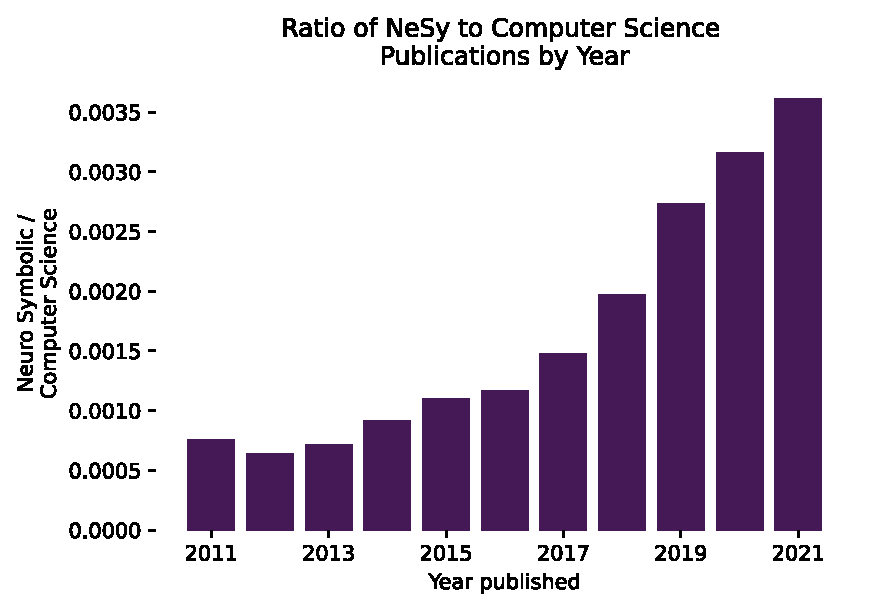
\includegraphics[width=.8\textwidth]{SW223228/allNesyByYear.eps}
    \source{\doi{10.3233/SW-223228}}
\end{frame}

\begin{frame}{Gartner -- Hype Cycle for Emerging Technologies, 2023}
    \centering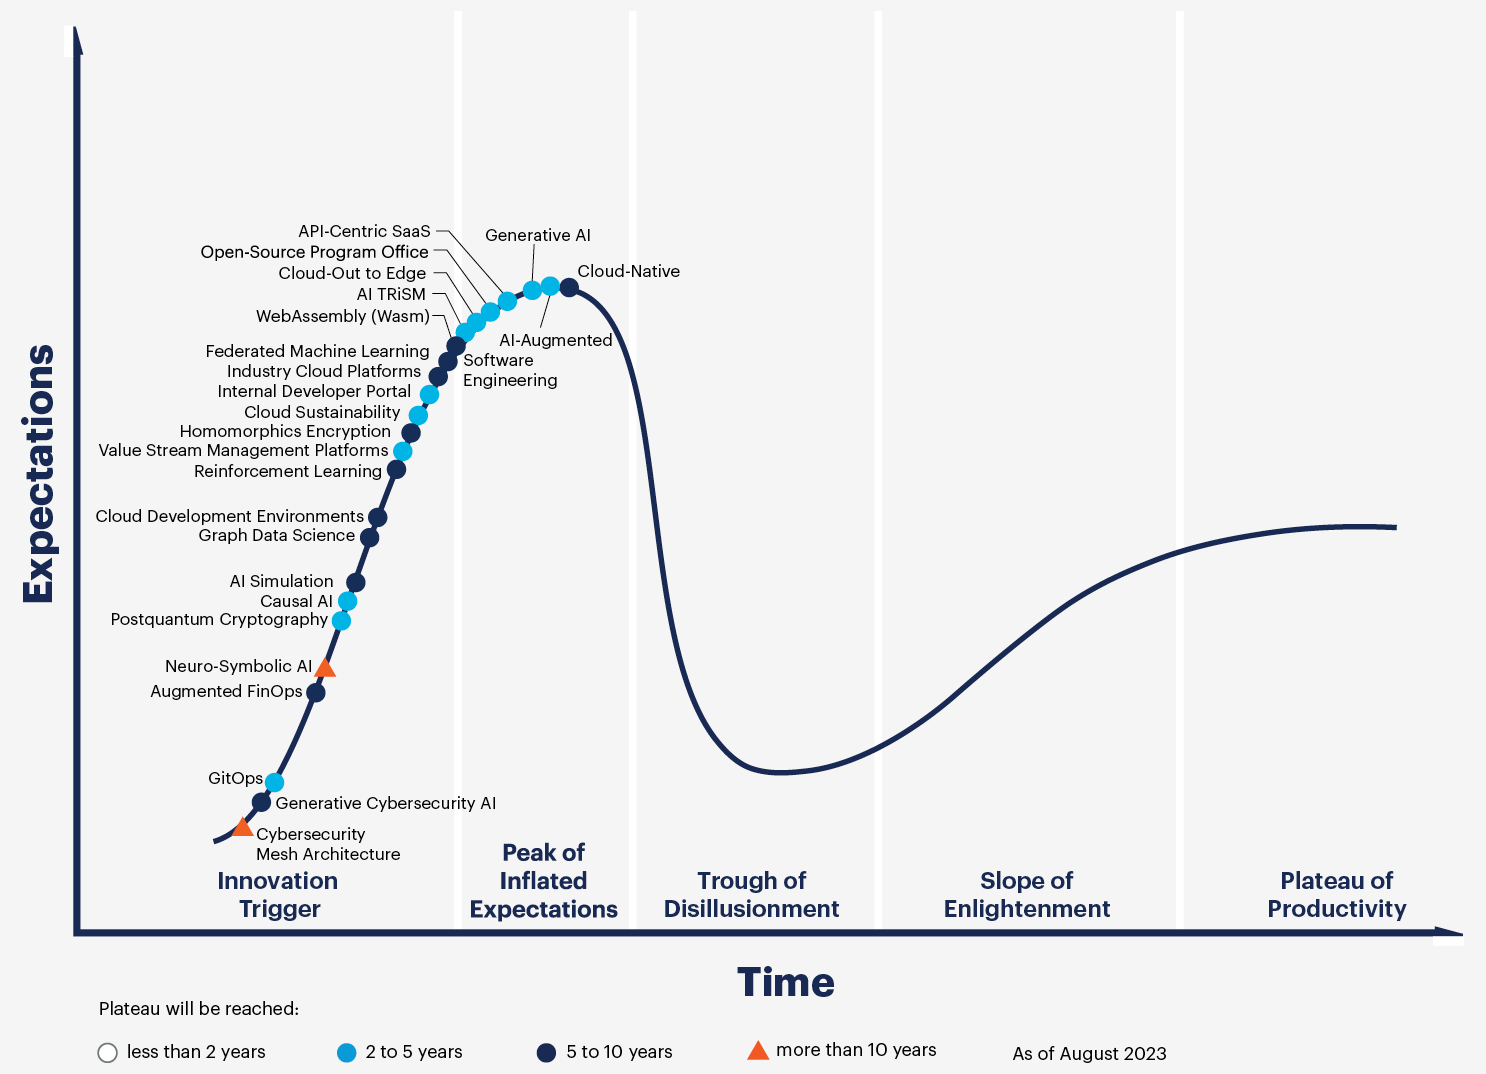
\includegraphics[width=.9\textwidth]{2023-gartner-hype-cycle-for-emerging-technologies.png}    
    \source{\url{https://www.gartner.com/en/articles/what-s-new-in-the-2023-gartner-hype-cycle-for-emerging-technologies}}
\end{frame}

\begin{frame}{Recent books}
    \begin{enumerate}
        \item Pascal Hitzler, Md. Kamruzzaman Sarker (eds.):
        \alert{Neuro-Symbolic} Artificial Intelligence: The State of the Art. Frontiers in Artificial Intelligence and Applications 342, IOS Press \alert{2021}, ISBN 978-1-64368-244-0
        \item Pascal Hitzler, Md. Kamruzzaman Sarker, Aaron Eberhart (eds.):
        Compendium of \alert{Neurosymbolic} Artificial Intelligence. Frontiers in Artificial Intelligence and Applications 369, IOS Press \alert{2023}, ISBN 978-1-64368-406-2
        \item Paulo Shakarian, Chitta Baral, Gerardo I. Simari, Bowen Xi, Lahari Pokala:
        \alert{Neuro Symbolic} Reasoning and Learning. Springer Briefs in Computer Science, Springer \alert{2023}, ISBN 978-3-031-39178-1
    \end{enumerate}
\end{frame}


\begin{frame}{Neuro-symbolic conferences and workshops}
    \begin{itemize}
        \item NeSy \url{https://people.cs.ksu.edu/~hitzler/nesy/}
        \begin{description}
            \item[2005--2022] an annual workshop affiliated with a major AI conference;
            \item[2023--] an annual conference of its own
        \end{description}             
        \item NeSy-GeMs (Neurosymbolic Generative Models) \url{https://nesygems.github.io/}
        \item GeNeSy (Generative Neuro-Symbolic AI) \url{https://sites.google.com/view/genesy2024/}
        \item many others, but not necessarily using this label
    \end{itemize}
\end{frame}

\begin{frame}{Other venues where NeSy topics were present}
    \begin{itemize}
        \item the International Conference on Machine Learning (ICML),
        \item  the Conference and Workshop on Neural Information Processing Systems (NeurIPS formerly NIPS),
        \item  the AAAI Conference on Artificial Intelligence (AAAI)
        \item  the International Joint Conference on Artificial Intelligence (IJCAI), and
        \item the International Conference on Learning Representations (ICLR).
    \end{itemize}
    \source{\url{https://arxiv.org/pdf/2105.05330.pdf}}
\end{frame}

\begin{frame}{A thriving community}
    We have a \alert{mailing list} and a \alert{Slack} of more than 900 members.

    \vspace{1cm}
    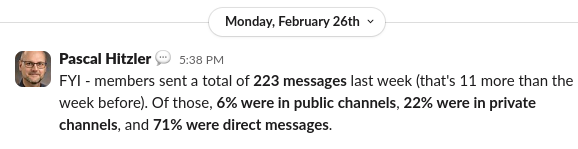
\includegraphics[width=\textwidth]{slack20240226.png}
\end{frame}

\begin{frame}{Many aliases}
    \centering
    \begin{tabular}{lll}
        
        Neural Terms & Symbolic Terms & Neuro-Symbolic Terms\\
        \hline
        sub-symbolic & symbolic & neuro-symbolic\\
        machine learning & reasoning & neural-symbolic \\
        deep learning & logic & neuro symbolic \\
         & & neural symbolic \\
         & & neurosymbolic \\
        
        \end{tabular}
        \pause

        \vspace{2cm}
        \alert{In truth, even more}
        \source{\doi{10.3233/SW-223228}}
\end{frame}

\begin{frame}{Different flavors of neuro-symbolic systems (axis 1)}
    \centering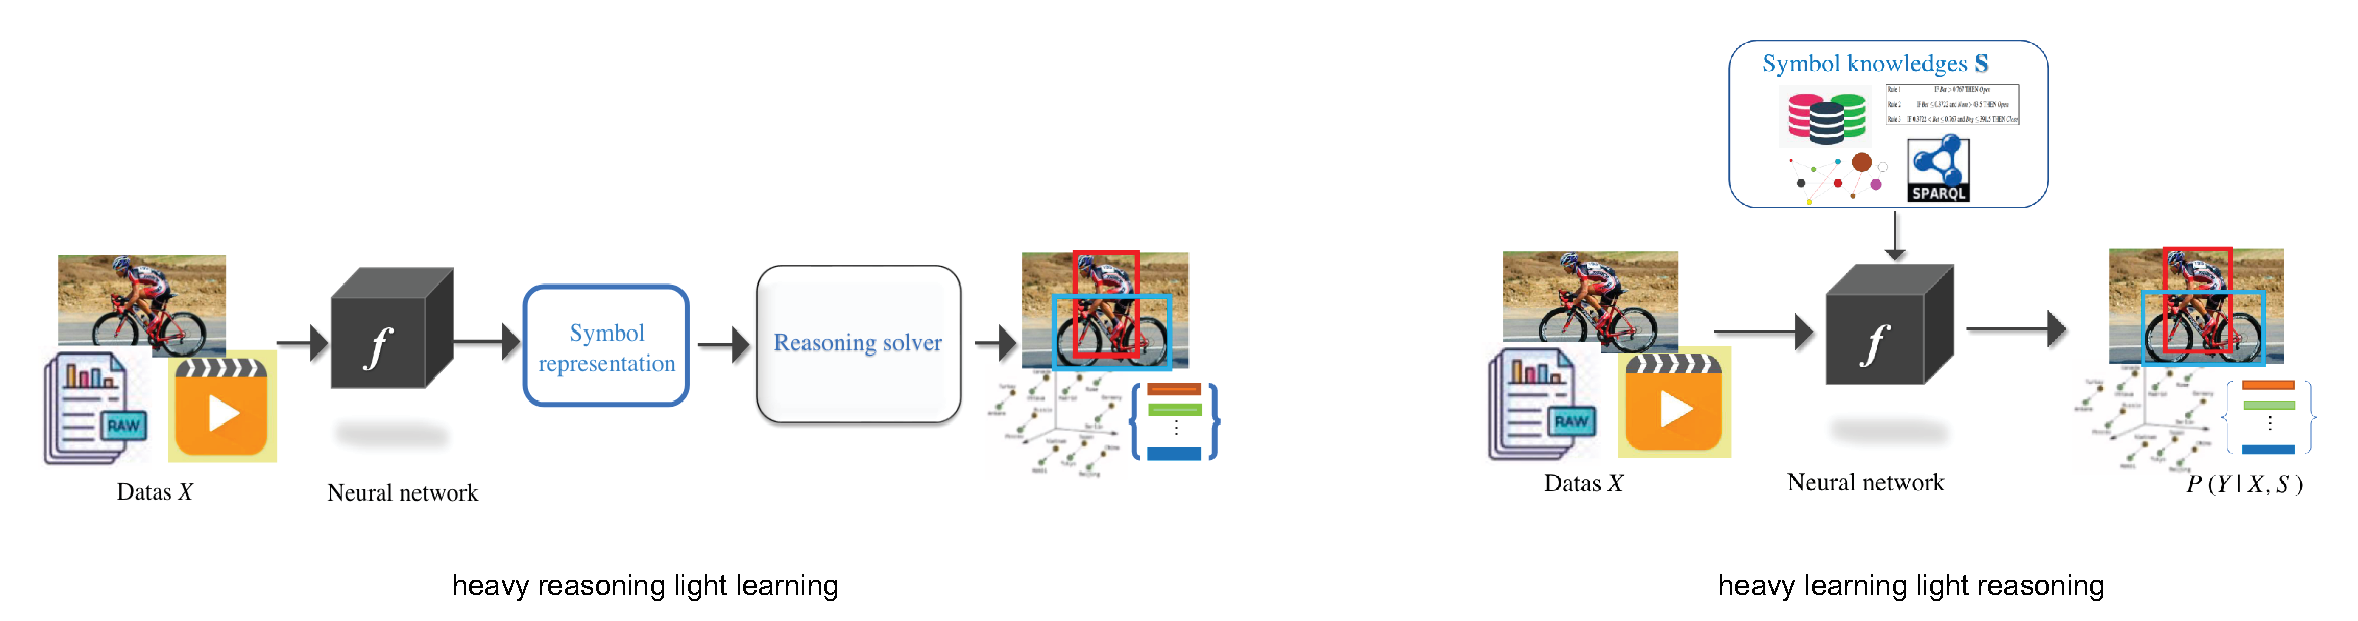
\includegraphics[width=.8\textwidth,clip,trim=0 0 18cm 3cm]{SW223228/yu-et-al.eps}\\
    \centering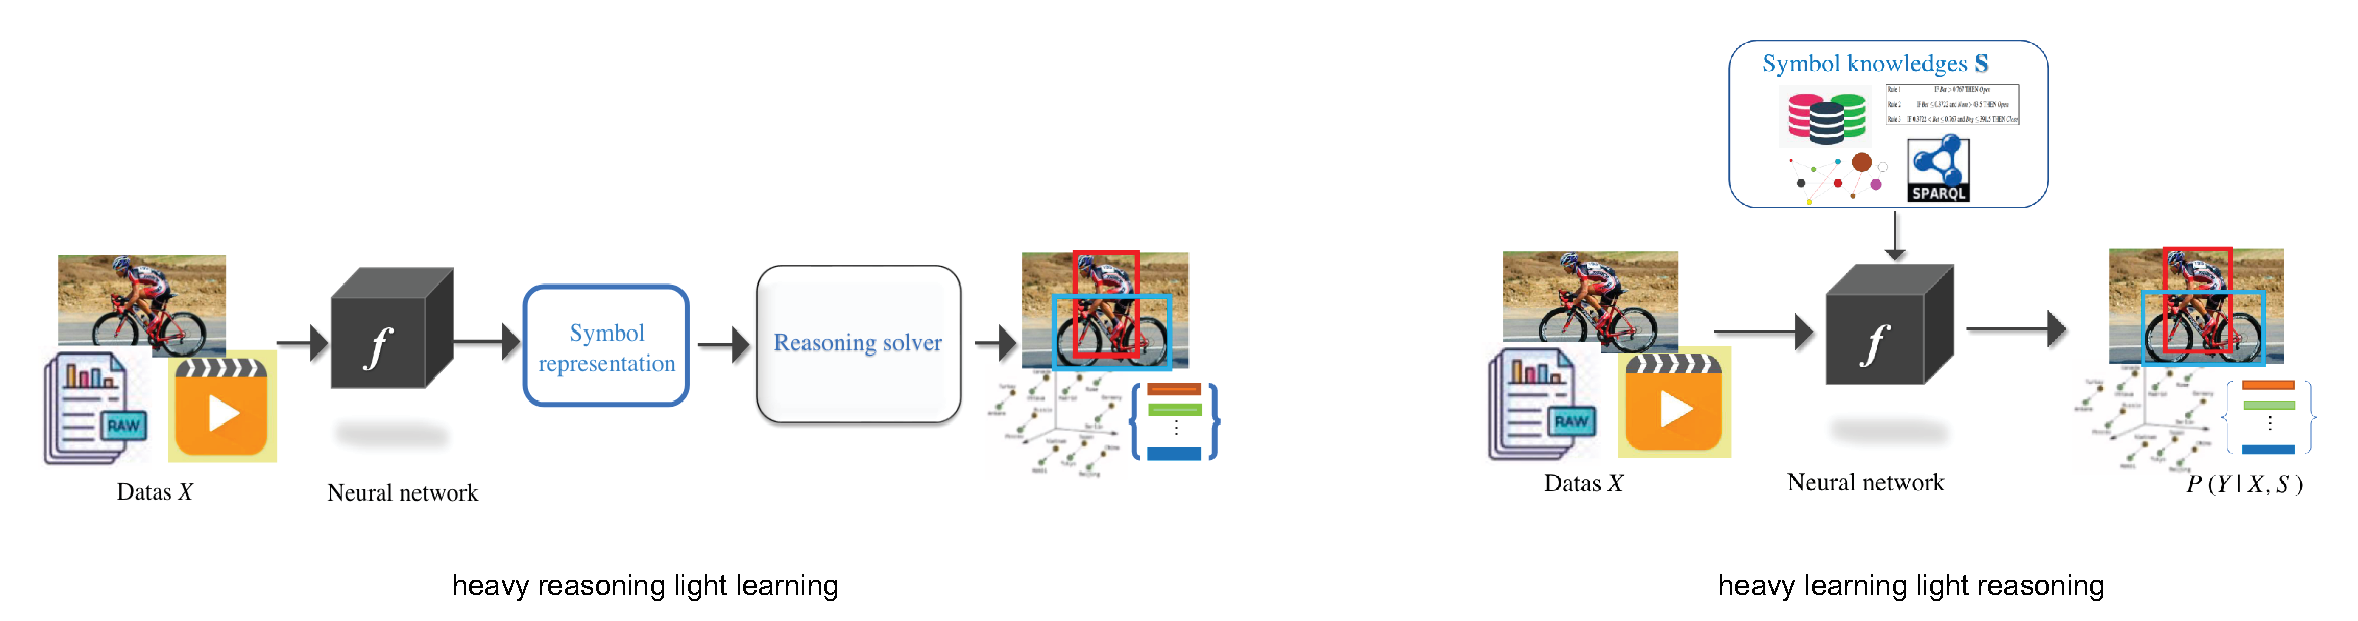
\includegraphics[width=.6\textwidth,clip,trim=23cm 0 0 0]{SW223228/yu-et-al.eps}
    \source{\doi{10.48550/ARXIV.2111.08164}}
\end{frame}


\begin{frame}{Different flavors of neuro-symbolic systems (axis 2)}
    \begin{itemize}
        \item Interrelation
            \begin{itemize}
                % integrated = end-to-end system
                % hybrid = dwa odrębne systemy luźno połączone
                \item Integrated versus hybrid
                % neuronal = inspiracja biologiczna, próba zrozumienia
                % connectionist = pragmatyczne wykorzystanie
                \item Neuronal versus connectionist
                % local = konkretne fragmenty neuronowe odpowiadaja konkretnym fragmentom symbolicznym
                % distributed = jak distributional semantics
                \item Local versus distributed
                % standard = real numbers, simple neurons, all neurons similar, simple recursive structures at the most
                % nonstandard = anything goes 
                \item Standard versus nonstandard
            \end{itemize}
            \item Language
                \begin{itemize}
                % symbolic = arbitrary system; as far as 1943
                % logical = wiadomo; as far as 1990
                \item Symbolic versus logical
                % propositional = rozumiane szeroko, ale generalnie skonczone logiki
                % first-order = infinite models, unifikacja itp
                \item Propositional versus first-order
                \end{itemize}
            \item Usage
                \begin{itemize}                
                \item Extraction versus representation
                \item Learning versus reasoning
                \end{itemize}
        \end{itemize}
    \source{\doi{10.48550/arXiv.cs/0511042} (a 2005 survey)}
\end{frame}

\begin{frame}{Different flavors of neuro-symbolic systems (axis 3)}
    \centering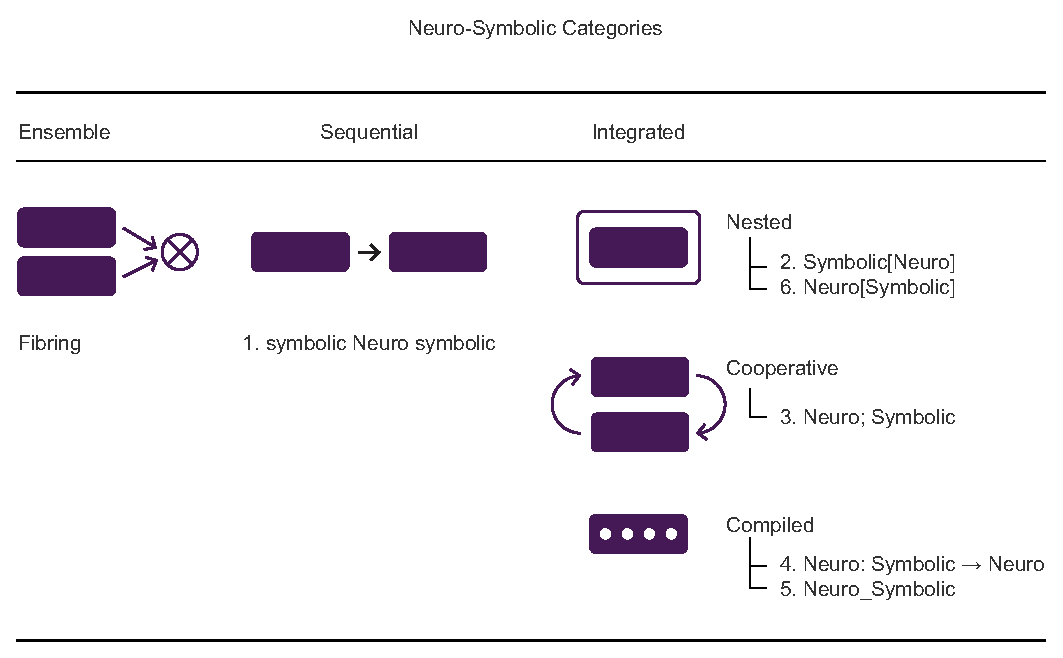
\includegraphics[width=.8\textwidth,clip,trim=3.5cm 0 0 0]{SW223228/Nesy-topology.eps}
    \source{\doi{10.3233/SW-223228}; Kautz @ AAAI-20}
    % Type 1 = standardowy DL
    % Type 2 = system symboliczny odwołujący się od systemu neuronowego
    % Type 3 = kooperacja
    % Type 4 = logika jako struktura sieci
    % Type 5 = logika jako ograniczenia (np. funkcja kosztu)
    % Type 6 = system neuronowy odwołujący się do systemu symbolicznego
\end{frame}

\begin{frame}{symbolic Neuro symbolic}
    \centering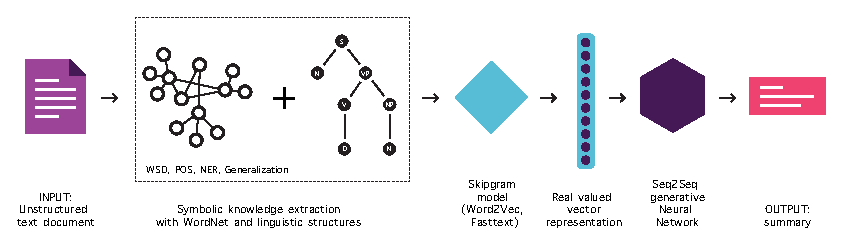
\includegraphics[width=\textwidth]{SW223228/Kouris_et_al.eps}
    \source{\doi{10.1162/coli_a_00417}}
\end{frame}

\begin{frame}{Symbolic[Neuro]}
    % Niektóre funkcje w DSL są realizowane komponentem neuronowym, np. LLM decyduje czy fragment tekstu pasuje do zadanego słowa kluczowego
    % transductive learning = soft labels wygenerowane przez grupę programów, które mają najlepsze wyniki na labeled webpages i zagregowanie wyników; ostatecznie wybierany jest ten, który ma najlepszy wynik na tak wygenerowanych soft labels
    \centering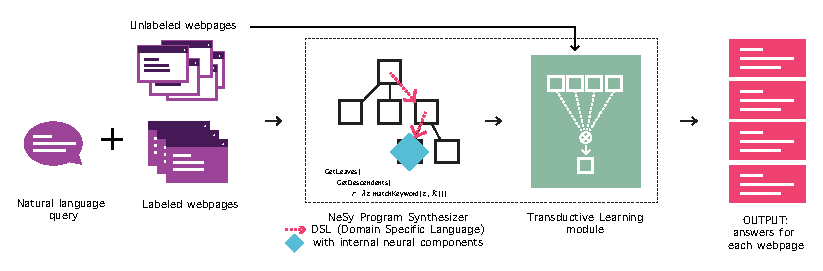
\includegraphics[width=\textwidth]{SW223228/chen_et_al.eps}
    \source{\doi{10.1145/3453483.3454047}}
\end{frame}

\begin{frame}{Symbolic[Neuro]}
    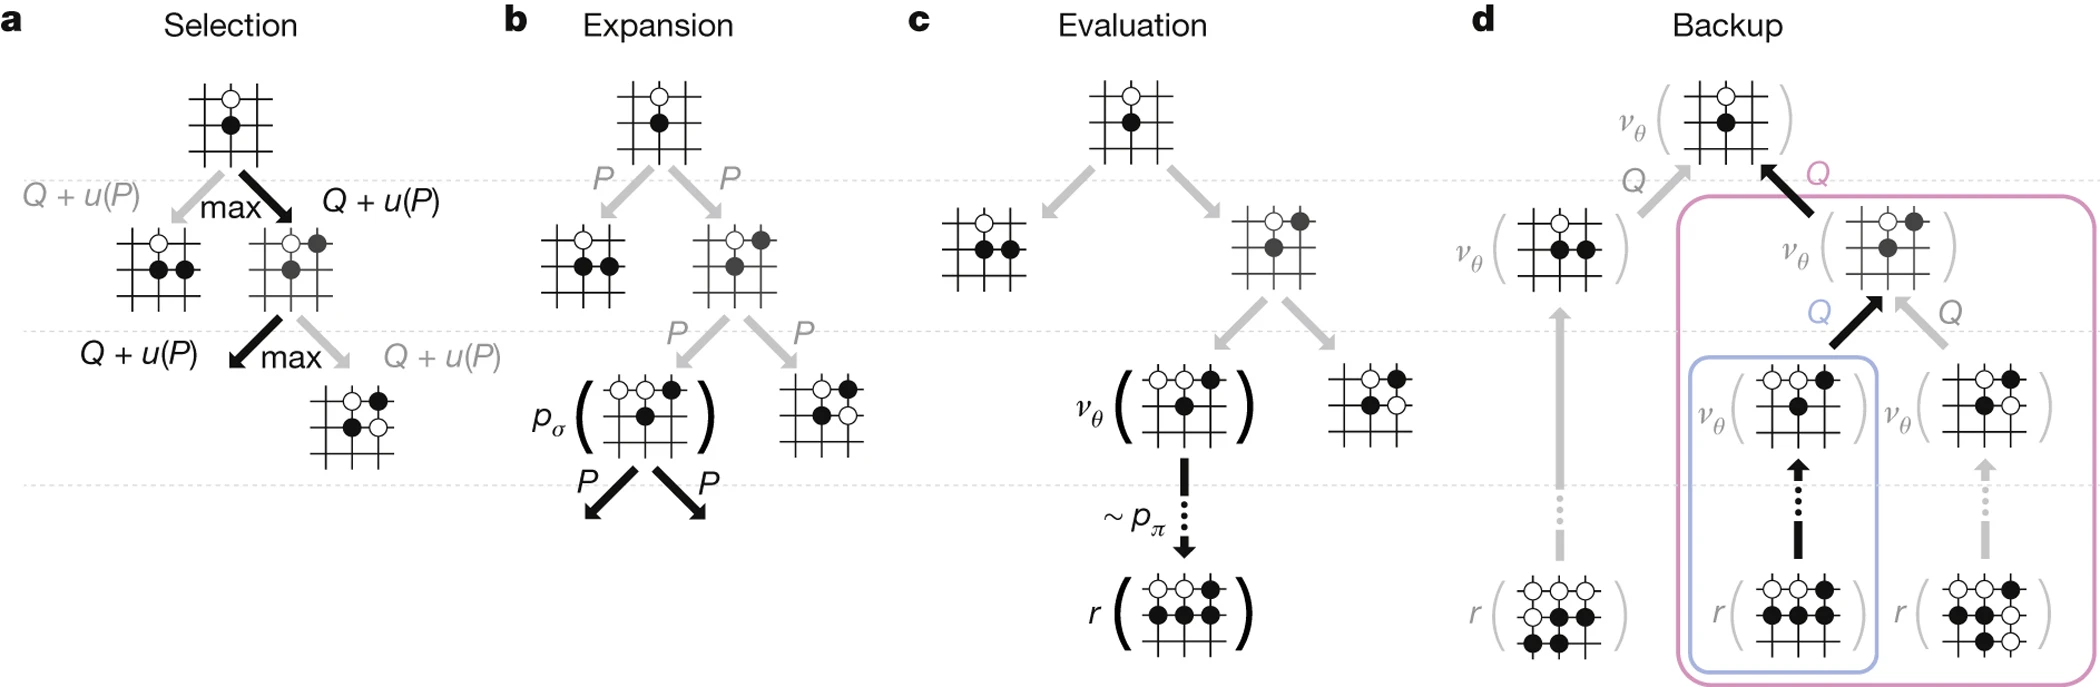
\includegraphics[width=\textwidth]{41586_2016_BFnature16961_Fig3_HTML.png}
    \source{AlphaGo \doi{10.1038/nature16961}}
\end{frame}

\begin{frame}{Neuro; Symbolic}
    % dwa neuronowe parsery, jeden do obrazow (zostaje w latent space), drugi do tekstu (tworzy DSL); wykonanie programów jest explicit, ale część operatorów jest neuronowa tzn. cecha jest reprezentowana w latent space, a porównanie 
    %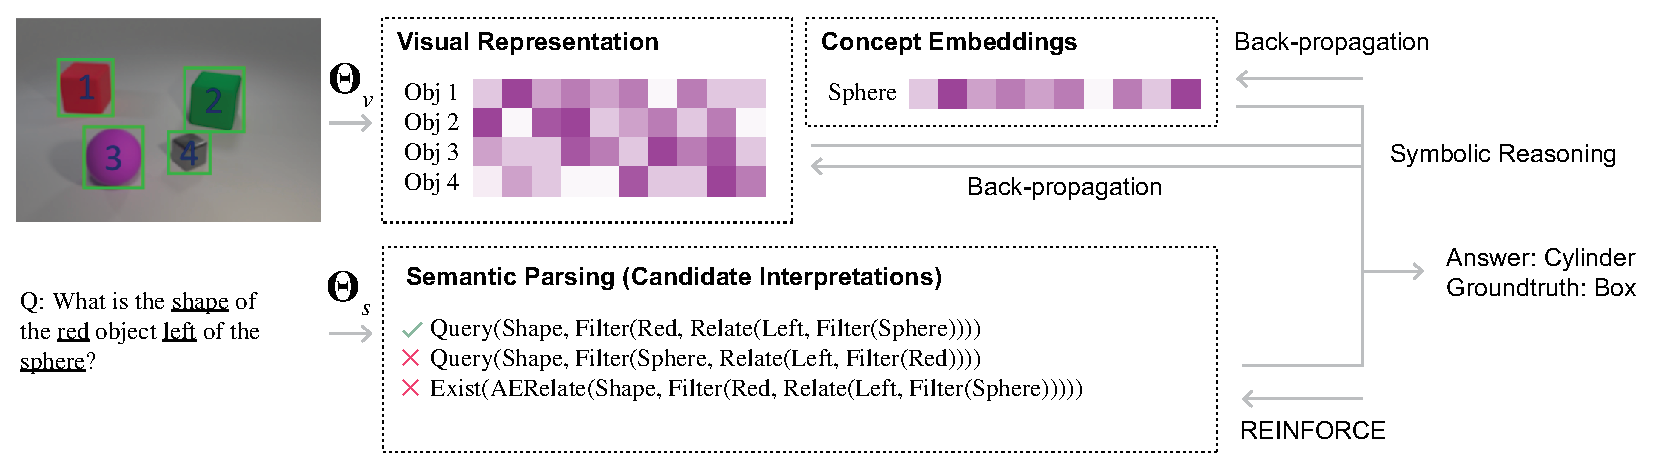
\includegraphics[width=\textwidth]{SW223228/mao_et_al.eps}
    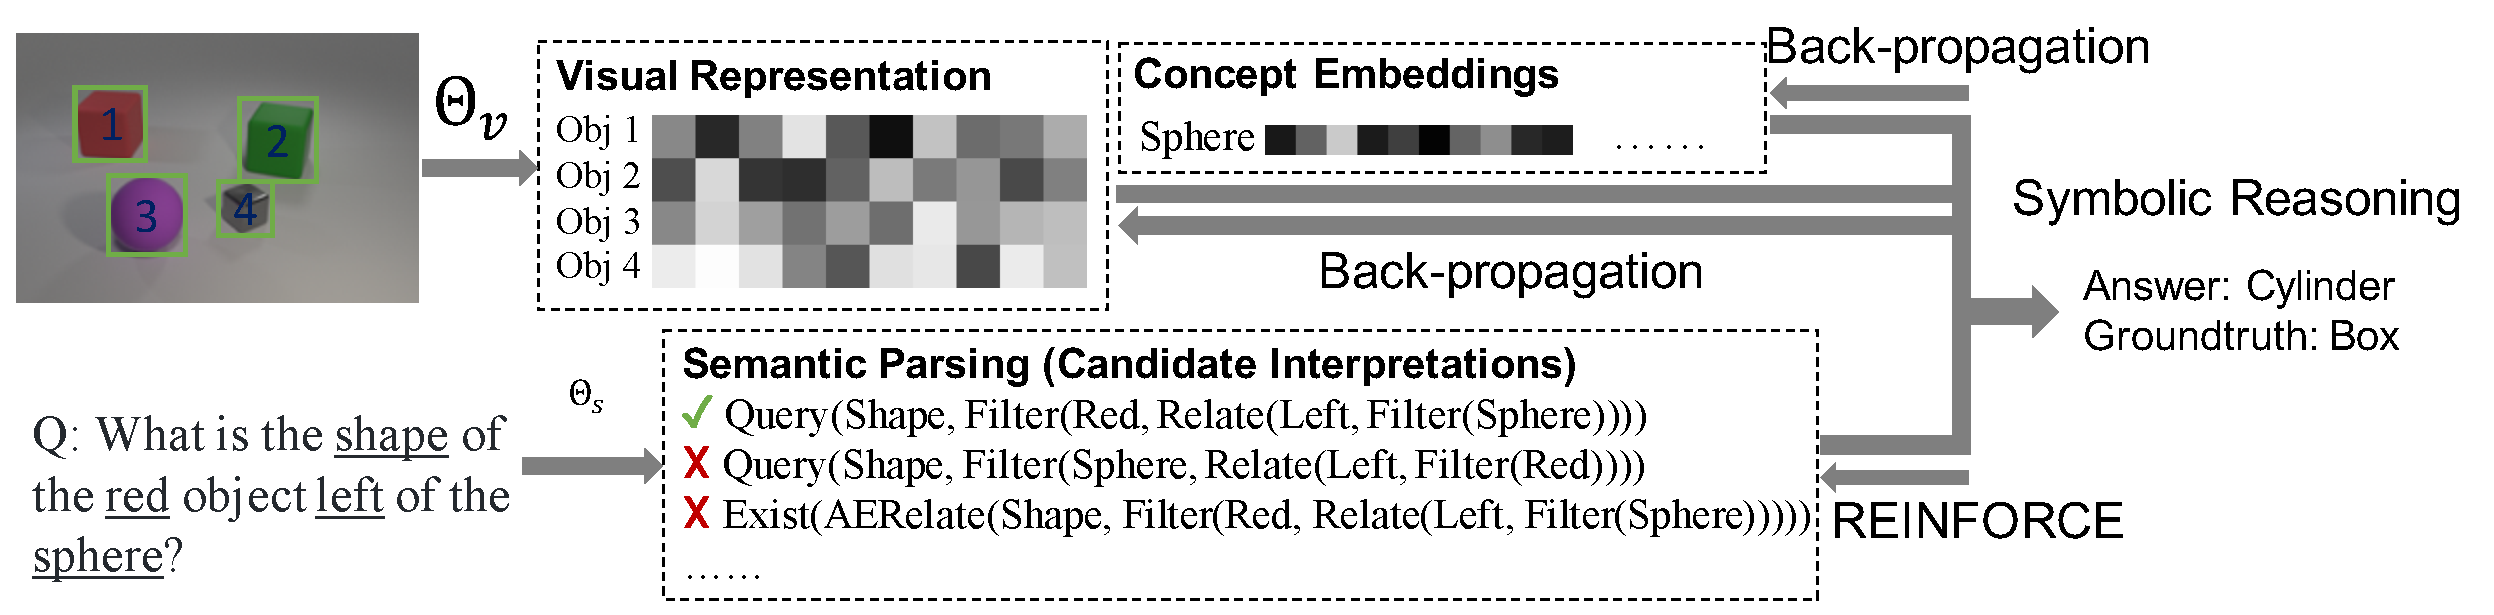
\includegraphics[width=\textwidth]{arXiv-1904.12584v1/raw/Framework.pdf}\\
    \vfill
    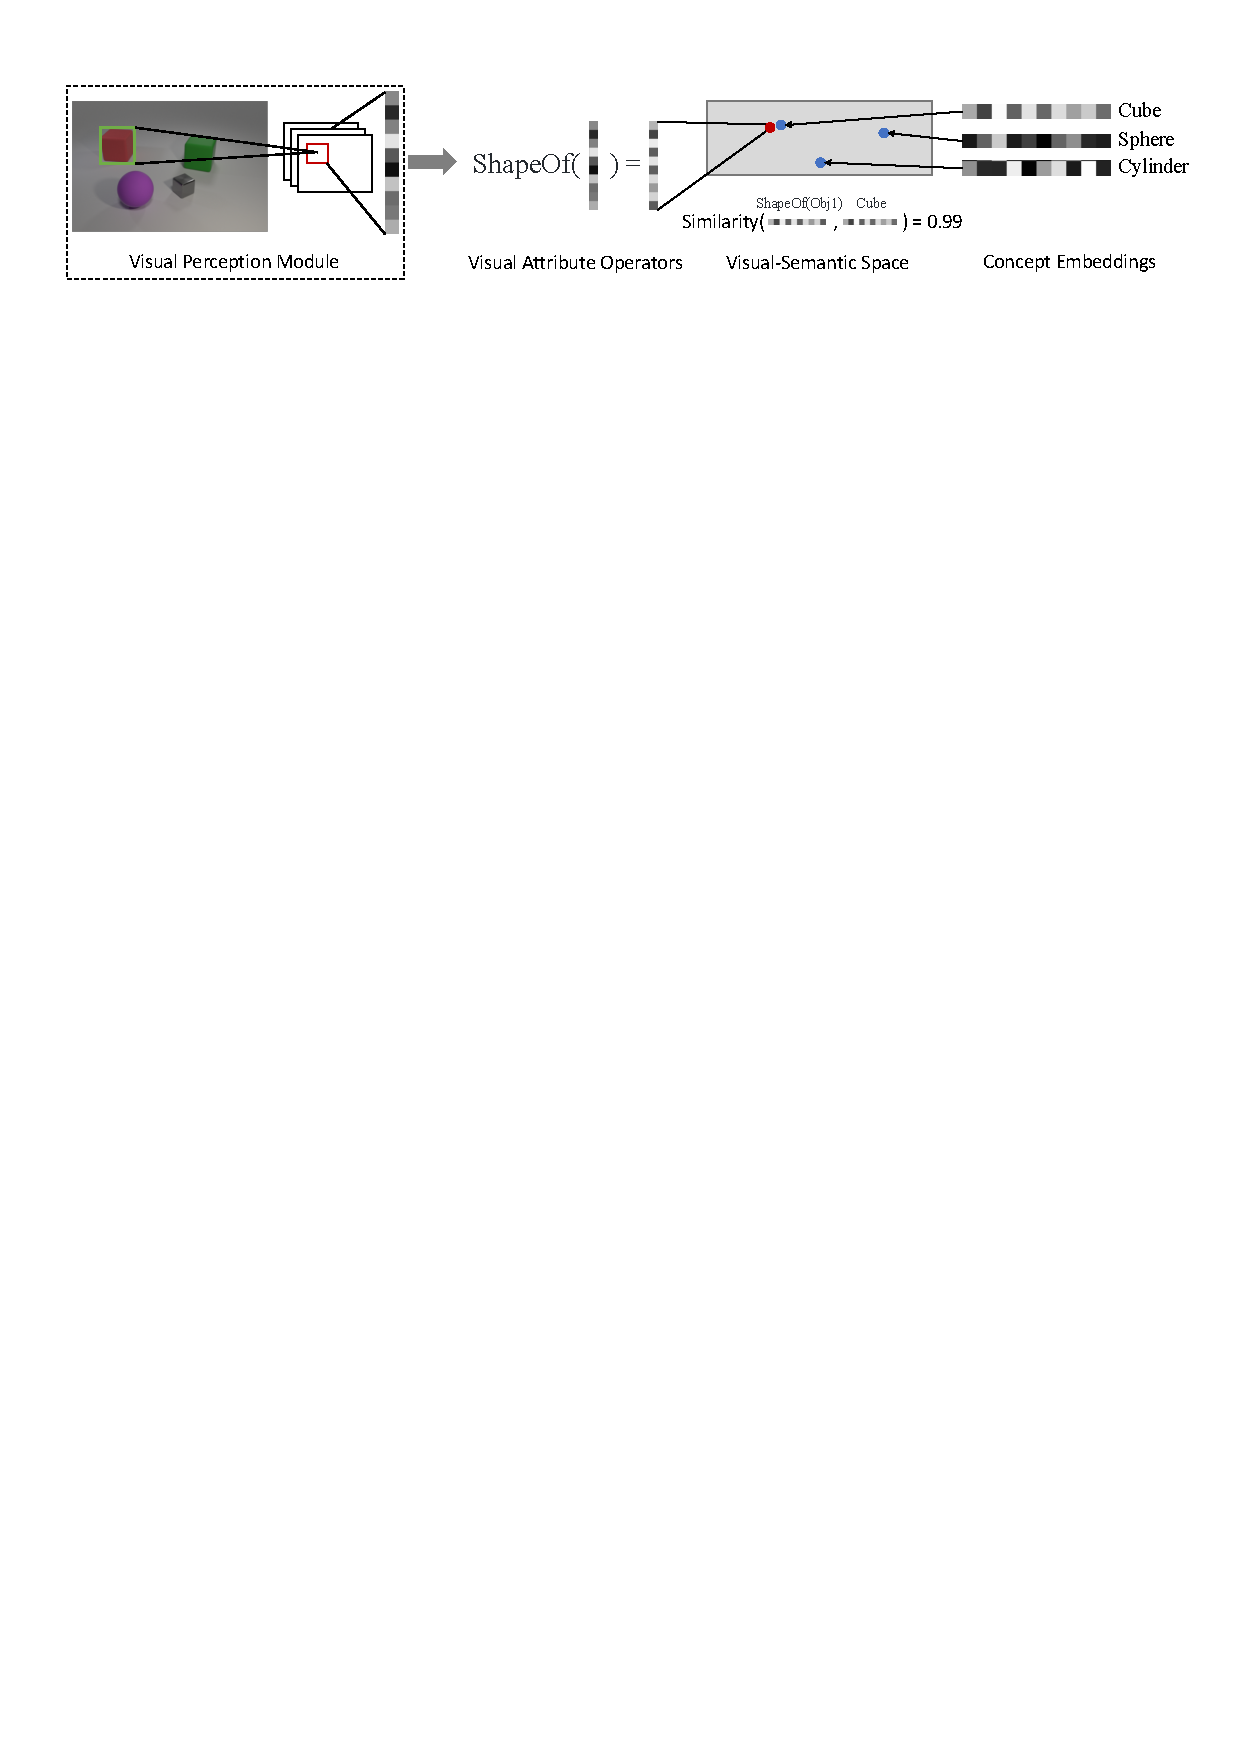
\includegraphics[width=\textwidth]{arXiv-1904.12584v1/raw/VSE.pdf}
    \source{The Neuro-Symbolic Concept Learner (NS-CL) \doi{10.48550/arXiv.1904.12584}}
\end{frame}

\begin{frame}{Neuro: Symbolic $\to$ Neuro}    
    % tekst jest zamienany keyword-based na ground facts
    % nauka w tradycyjnym reinforcement learning, zeby miec policy
    % ekstrakcja reguł z policy przez wykorzystanie go jako teacher; w tym procesie optymalizowane są wagi pokazane na rysunku, które reprezentują taką niby-rozmytą logikę
    \centering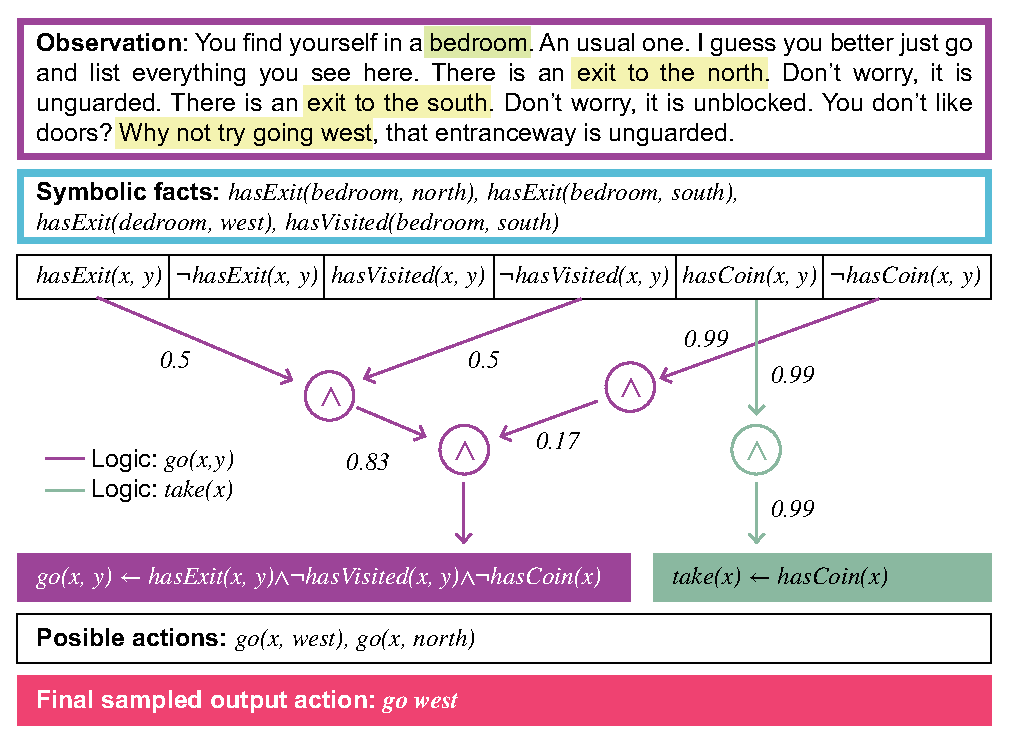
\includegraphics[width=.9\textwidth]{SW223228/slate-neuro-symbolic-type-4.eps}
    \source{SLATE \doi{10.18653/v1/2021.emnlp-main.245}}
\end{frame}

\begin{frame}{Neuro: Symbolic $\to$ Neuro}
    % wiedza symboliczna (o czestosci wspolwystepowania) jest zamieniana w architekture sieci
    %1) employing symptom and disease embedding as an input vector; 2) using basic triple knowledge to determine the connectivity from the input layer to the shallow logic layer 
%; 3) constructing a Huffman tree based on the frequency of knowledge to represent the deep logic knowledge. 4) using each node vector as features for a softmax classifier
    \centering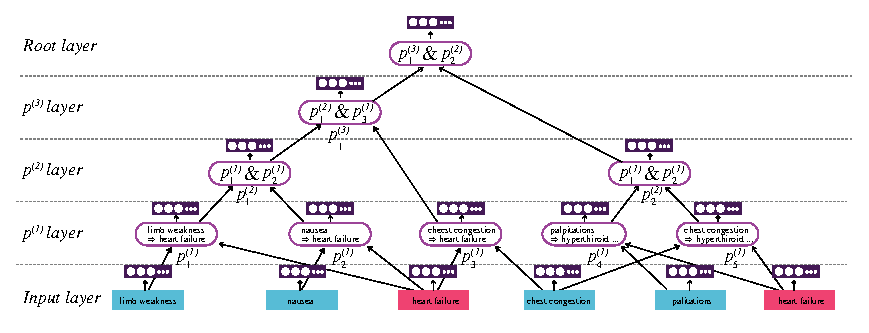
\includegraphics[width=\textwidth]{SW223228/neuro-symbolic-huffman-tree.eps}
    \source{\doi{10.1016/j.artmed.2019.101772}}
\end{frame}

\begin{frame}{Neuro\textsubscript{Symbolic}}
    % Wiedza tekstowa jest anotowana i trenowane sa embeddingi, ktore nastepnie sa laczone z wiedza strukturalna reprezentowana jako Logical Tensor Network; to pozwala np. odpytywac model o informacje na temat encji ktorych nie bylo w bazie wiedzy, ale znana jest dla nich reprezentacja embeddingowa i ktore sa podobne do encji, ktore w bazie wiedzy sa    
    \centering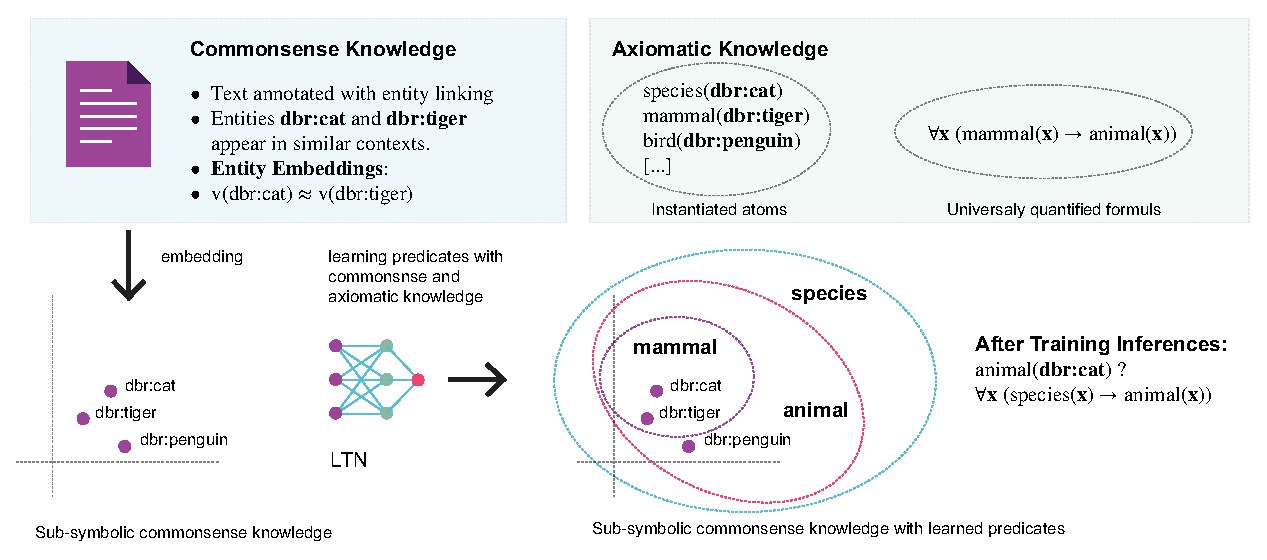
\includegraphics[width=\textwidth]{SW223228/bianchi2019.eps}
    \source{\doi{10.1007/978-3-030-31095-0\_11}}
\end{frame}

\begin{frame}{Neuro[Symbolic]}
    \begin{block}{\doi{10.3233/SW-223228}}
        Type 6 Neuro[Symbolic] is the most tightly integrated but perhaps the most elusive as there do not appear to be
any recent implementations in existence. According to Kautz, this is the ultimate NeSy system which should be
capable of efficient combinatorial reasoning at the level of super-intelligence, if not human intelligence.
    \end{block}
    \pause
    \vspace{1cm}
    ChatGPT and the like with external functions?
\end{frame}

\begin{frame}{A disclaimer}
    These classifications are not necessarily comprehensive nor the values are disjoint.
    They are only useful labels for \alert{clusters}, not a noise-free classification task.
\end{frame}

\end{document}
